\chapter{Path Planning Algorithm}

The path planning algorithm implemented in this project was the Game-Theoretic Optimal Deformable Zone with Inertia and Local Approach (GODZILA) algorithm. This potential fields algorithm uses the closed form formulation of an optimized cost function that rewards motion towards a goal location and penalizes motion towards obstacles and in directions other than the current heading. In addition to the optimized cost function, GODZILA incorporates a straight line path planner when the goal is in sight of the robot and a randomization function to allow the robot to escape local minima.

Using the closed form formulation of the cost function in quadratic terms, the algorithm effectively generates forces that push the robot from obstacles and pull it towards the goal. The component penalizing motion in directions other than the current heading of the robot acts like an inertia term which helps prevent oscillations and forces any limit cycles to be larger, which helps eliminate certain local minima.

Occlusion forces are generated through use of sensor data from the robot's distance sensors. Each distance reading is used to generate a force magnitude which is applied as a vector to the robot along the orientation of the sensor relative to the robot.
The goal force is generated in the same manner, with estimated distance to the goal generating a magnitude applied to the vector along the estimated orientation of the goal relative to the robot. The inertia term provides a constant bias towards the current heading of the robot. 

\begin{figure}[h]
	\centering
	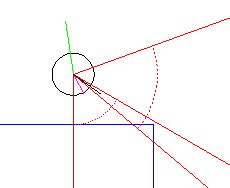
\includegraphics{force_sim1.jpg}
	\caption[Simulation showing component forces.]
	{Simulation showing component forces. The green line shows the summed occlusion vectors, magenta is the goal vector,
	 black is the inertia vector.}
	\label{fig:forceSim1}
\end{figure}

The angle from the sum of these forces is then taken as the desired heading of the robot and converted into an angular rate with is passed to the vehicle.